% ===========================================================================
\section{New algorithm: SeaSel}\label{sec:algo}
% ===========================================================================
Algorithm~1 summarises SeaSel. It has three phases. In the offline phase, an ensemble of physics-biased attention networks is trained on logged epochs $\mathcal D_{\rm tr}$ with a multi-task loss that predicts aggressive and robust success (Section~\ref{sec:arch}), and a temperature is fitted on a validation split. In the calibration phase, a held-out set $\mathcal D_{\rm cal}$ of $n$ epochs is used to certify a pair $(\hat\gamma,\hat\lambda)$ by Learn-then-Test (Section~\ref{sec:uq}). In the deployment phase, the gateway evaluates the ensemble once per epoch, applies the certified rule (\ref{eq:accept}), transmits and, when acknowledgements reveal drift, updates the threshold online.

\begin{center}
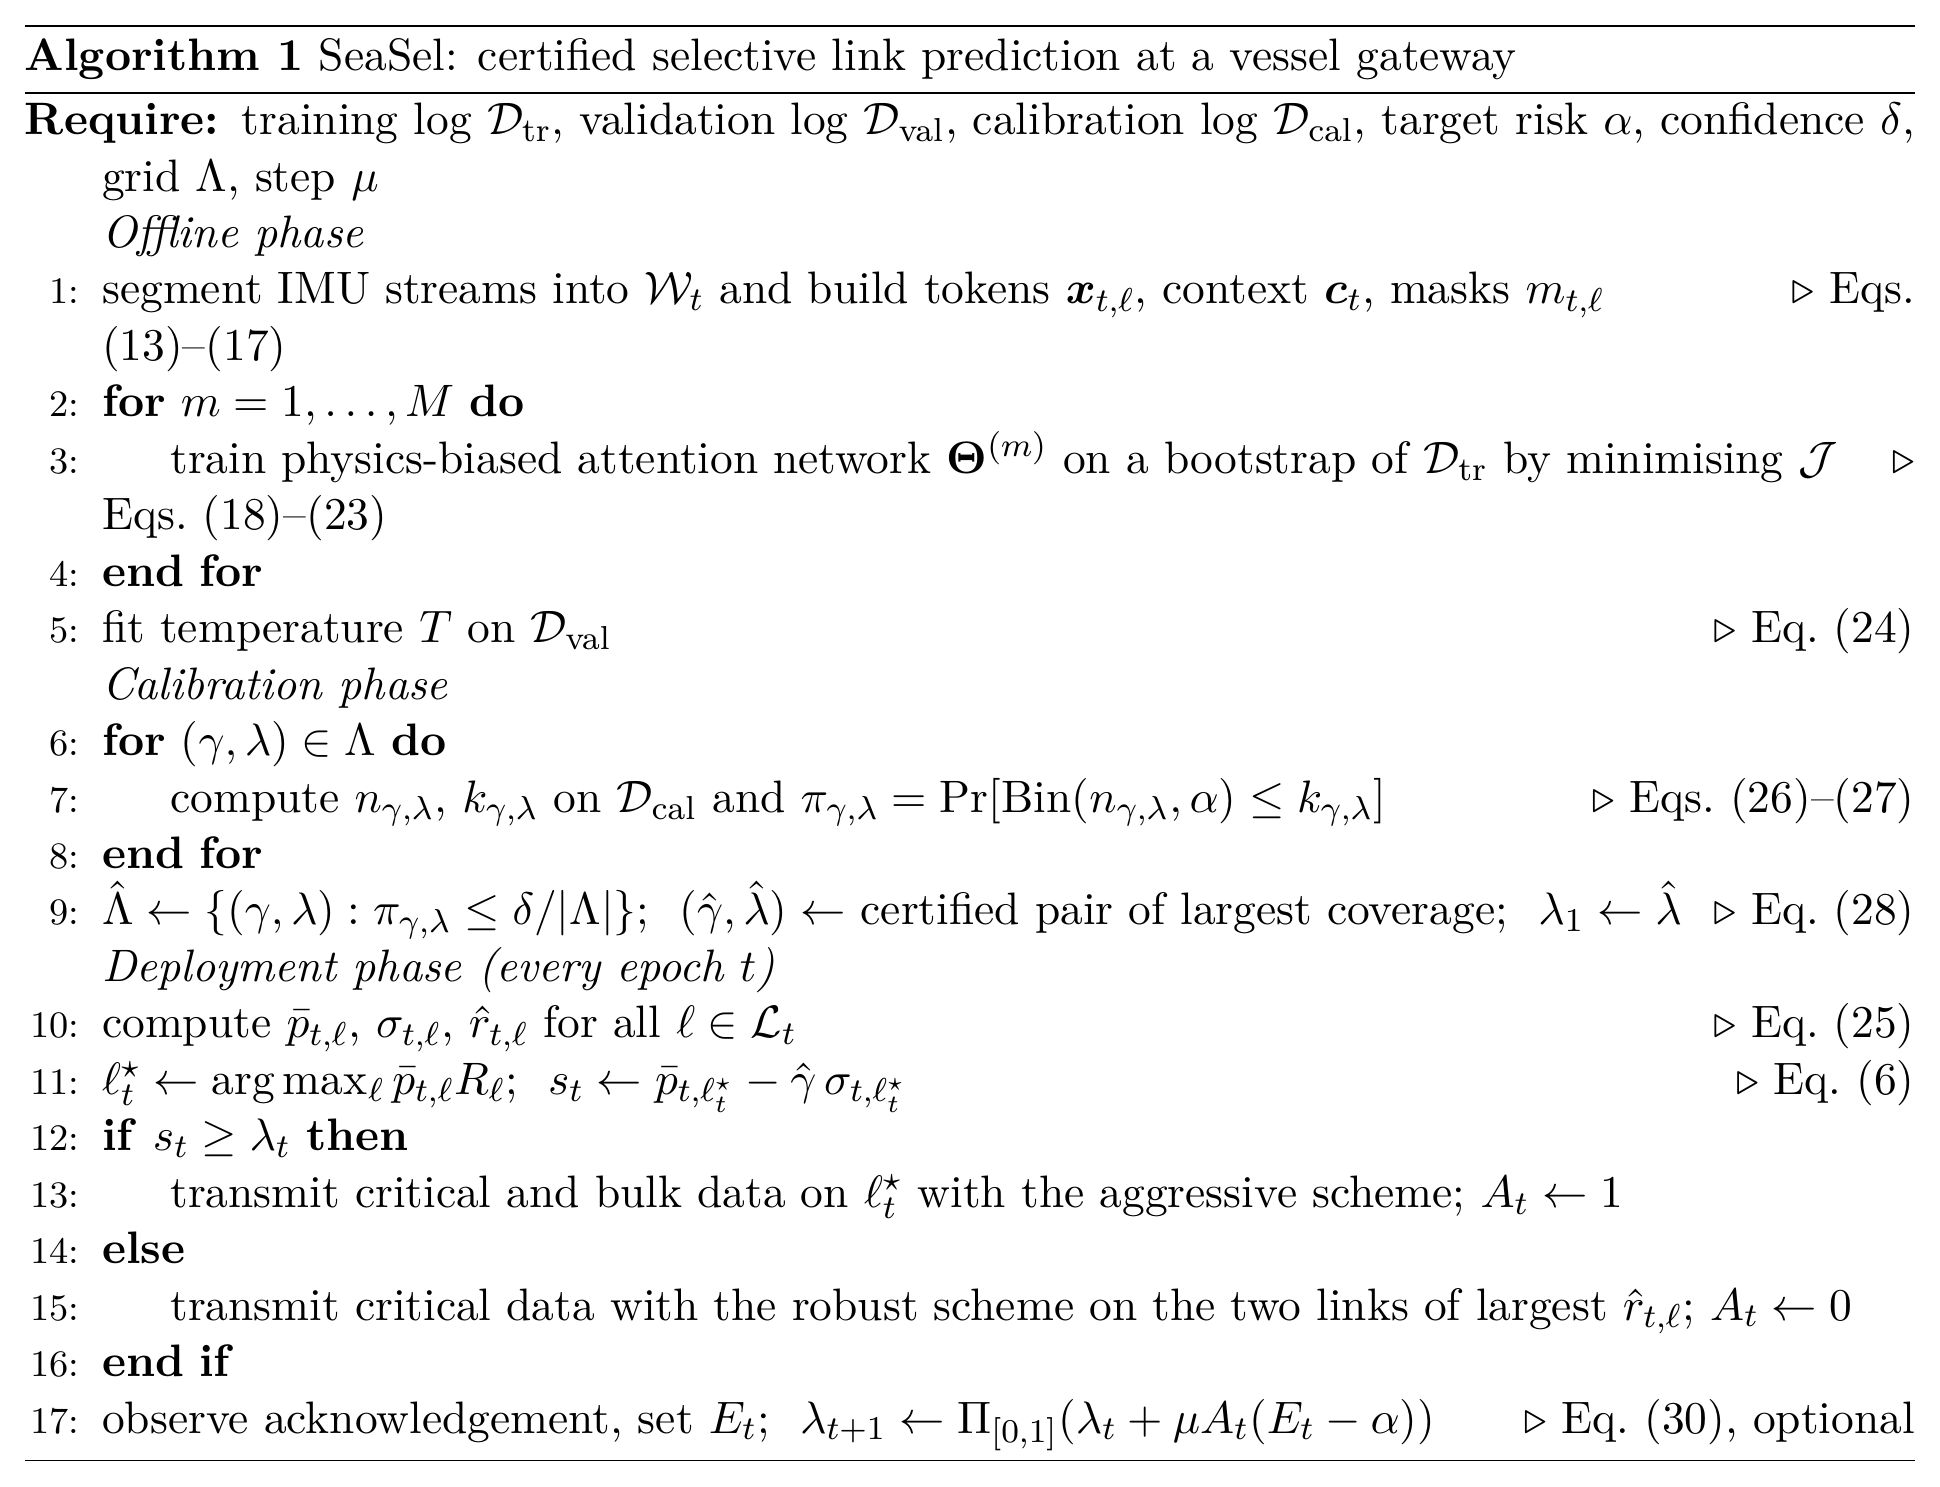
\includegraphics[width=0.97\textwidth]{../figures/diagrams/algorithm.png}
\end{center}

The certification step rests on the following result.

\begin{theorem}[Certified selective risk]\label{thm:cert}
Let the calibration epochs and a test epoch be independent and identically distributed, and let $\Lambda$ be a finite grid of $(\gamma,\lambda)$ pairs. For each pair, let $n_{\gamma,\lambda}$ be the number of accepted calibration epochs and $k_{\gamma,\lambda}$ the number of aggressive failures among them. Define the p-value $\pi_{\gamma,\lambda}=\Pr[\mathrm{Bin}(n_{\gamma,\lambda},\alpha)\le k_{\gamma,\lambda}]$ and the certified set $\hat\Lambda=\{(\gamma,\lambda)\in\Lambda:\pi_{\gamma,\lambda}\le\delta/|\Lambda|\}$. Then any pair selected from $\hat\Lambda$, in particular the one maximising calibration coverage, satisfies $\Pr[R_{\rm sel}(\hat\gamma,\hat\lambda)\le\alpha]\ge1-\delta$.
\end{theorem}
\noindent\textit{Proof.} Fix $(\gamma,\lambda)$ with $R_{\rm sel}(\gamma,\lambda)>\alpha$. Conditionally on $n_{\gamma,\lambda}$, the accepted calibration epochs are independent draws from the distribution conditioned on $\{s_t(\gamma)\ge\lambda\}$, so $k_{\gamma,\lambda}\sim\mathrm{Bin}(n_{\gamma,\lambda},R_{\rm sel})$, which stochastically dominates $\mathrm{Bin}(n_{\gamma,\lambda},\alpha)$. Hence $\Pr[\pi_{\gamma,\lambda}\le u]\le u$ for all $u$, so $\pi_{\gamma,\lambda}$ is a valid p-value. By the union bound over the at most $|\Lambda|$ pairs whose null hypothesis is true, the probability that any of them enters $\hat\Lambda$ is at most $\delta$. On the complementary event every certified pair has $R_{\rm sel}\le\alpha$, whatever rule is then used to choose among them\cite{angelopoulos2025,bates2021}. $\square$

\begin{proposition}[Service-level guarantee]\label{prop:service}
On the event of Theorem~\ref{thm:cert}, the critical-message miss rate obeys (\ref{eq:missbound}). If, in addition, the fallback failure probability satisfies $\rho_F\le\rho$, then $\mathcal M\le\alpha c+\rho(1-c)\le\max(\alpha,\rho)$, and the goodput satisfies $\mathcal G\ge T_x\big[c(1-\alpha)\min_\ell R_\ell+(1-c)(1-\rho)R_0\big]$.
\end{proposition}
\noindent\textit{Proof.} Equation~(\ref{eq:miss}) gives $\mathcal M=c\,R_{\rm sel}+(1-c)\rho_F$; substituting $R_{\rm sel}\le\alpha$ and $\rho_F\le\rho$ yields both inequalities. Equation~(\ref{eq:goodput}) is bounded in the same way term by term. $\square$

The calibration cost is $O(|\Lambda|\,n)$ and is performed once per calibration window. The deployment cost per epoch is one forward pass of $M$ small networks over at most $K+1$ tokens, which is dominated by the attention product and scales as $O(M K^2 d)$, with $d$ the model width.

% ===========================================================================
\section{Preprocessing, segmentation, and input representation}\label{sec:prep}
% ===========================================================================
\textbf{Segmentation.} The inertial measurement unit samples roll $\phi$ and pitch $\vartheta$ at $f_s=2$\,Hz. For epoch $t$ the gateway extracts the segment immediately preceding the decision,
\begin{equation}\label{eq:segment}
\mathcal W_t=\big\{(\phi(\tau),\vartheta(\tau)):\ t\Delta-w\le\tau<t\Delta\big\},\qquad w=60\ {\rm s},
\end{equation}
so no information from the transmission itself leaks into the input. Each segment is summarised by root-mean-square motion and angular rate,
\begin{equation}\label{eq:rms}
\bar\phi_t=\Big(\tfrac1{|\mathcal W_t|}\textstyle\sum_{\mathcal W_t}\phi^2\Big)^{1/2},\quad
\bar\vartheta_t=\Big(\tfrac1{|\mathcal W_t|}\textstyle\sum_{\mathcal W_t}\vartheta^2\Big)^{1/2},\quad
\omega_t=f_s\Big(\tfrac1{|\mathcal W_t|}\textstyle\sum_{\mathcal W_t}(\Delta\phi)^2+(\Delta\vartheta)^2\Big)^{1/2},
\end{equation}
and by the dominant motion period obtained from the periodogram of the roll signal:
\begin{equation}\label{eq:period}
P_t=\Big(\arg\max_{f>0}\left|\textstyle\sum_{\tau\in\mathcal W_t}(\phi(\tau)-\bar\phi^{\rm m}_t)e^{-j2\pi f\tau}\right|^2\Big)^{-1},
\end{equation}
where $\bar\phi^{\rm m}_t$ is the segment mean. The rain-gauge reading is log-compressed, $\tilde R_t=\log(1+R_t)+\epsilon_t$ with sensor noise $\epsilon_t$.

\textbf{Input representation.} The vessel context is $\bm c_t=[\bar\phi_t,\bar\vartheta_t,\omega_t,P_t,\tilde R_t,v_t,\log(1+d^{\rm port}_t)]$, where $v_t$ is the ship speed and $d^{\rm port}_t$ the distance to the nearest port. Each candidate link becomes a token
\begin{equation}\label{eq:token}
\bm x_{t,\ell}=\Big[\tfrac{\theta_{t,\ell}}{90},\sin\psi^{\rm r}_{t,\ell},\cos\psi^{\rm r}_{t,\ell},\dot\theta_{t,\ell},\log(1+\tau^{\rm set}_{t,\ell}),\tfrac{\chi^0_{t,\ell}}{90},e^{\rm sec}_{t,\ell},\tfrac{\Delta^{\rm b}_{t-1,\ell}}{10},h_{t,\ell},\iota_{t,\ell},\log(1+d_{t,\ell}),\tfrac{\mathrm{SNR}^{\rm cs}_{t,\ell}}{10}\Big],
\end{equation}
containing the elevation, the azimuth $\psi^{\rm r}$ relative to the heading, the elevation rate, the time to setting from the ephemeris, the scan angle on a level deck, an exponentially weighted blockage evidence for the azimuth sector, the last observed beacon deficit $\Delta^{\rm b}$ (clear-sky prediction minus measured beacon SNR) with its availability flag $h$, a coastal-link indicator $\iota$, the range and the clear-sky SNR. The unit direction $\bm u_{t,\ell}$ is kept separately for the attention bias. Up to $K=8$ satellites ordered by elevation and one coastal token form a padded set with mask $m_{t,\ell}\in\{0,1\}$.

\textbf{Normalisation.} With mean $\mu_j$ and standard deviation $s_j$ of feature $j$ computed over valid training tokens only, every feature is standardised and masked:
\begin{equation}\label{eq:norm}
\tilde x_{t,\ell,j}=m_{t,\ell}\,\frac{x_{t,\ell,j}-\mu_j}{s_j},
\end{equation}
and missing values (sensor dropouts) are set to the training mean, i.e.\ zero after standardisation. Training, validation and calibration splits are formed by vessel, so that no vessel contributes to both training and evaluation.

% ===========================================================================
\section{Proposed attention-enhanced maritime IoT satellite architecture}\label{sec:arch}
% ===========================================================================
Each token is first embedded together with the vessel context,
\begin{equation}\label{eq:embed}
\bm h^{0}_{t,\ell}=\mathrm{ReLU}\big(\bm W_1[\tilde{\bm x}_{t,\ell};\tilde{\bm c}_t]+\bm b_1\big)\in\mathbb R^{d}.
\end{equation}
The key element is a self-attention layer over the candidate set whose logits contain a geometric prior. Links that point to nearby directions share rain cells, blockage sectors and motion-induced scan loss, so the attention logit between links $\ell$ and $k$ is
\begin{equation}\label{eq:pba}
e_{\ell k}=\frac{(\bm W_q\bm h^0_{t,\ell})^{\top}(\bm W_k\bm h^0_{t,k})}{\sqrt{d_k}}-\operatorname{softplus}(\beta)\big(1-\bm u_{t,\ell}^{\top}\bm u_{t,k}\big)+\log m_{t,k},
\end{equation}
where $\beta$ is learned and $\log m_{t,k}=-\infty$ removes padded tokens. The attention weights and the updated representation are
\begin{equation}\label{eq:softmax}
a_{\ell k}=\frac{\exp e_{\ell k}}{\sum_{k'}\exp e_{\ell k'}},\qquad
\bm h^{1}_{t,\ell}=\bm h^{0}_{t,\ell}+\bm W_o\sum_k a_{\ell k}\bm W_v\bm h^{0}_{t,k},
\end{equation}
followed by a residual feed-forward block
\begin{equation}\label{eq:ffn}
\bm h^{2}_{t,\ell}=\bm h^{1}_{t,\ell}+\bm W_3\,\mathrm{ReLU}\big(\bm W_2\bm h^{1}_{t,\ell}+\bm b_2\big).
\end{equation}
Because (\ref{eq:pba})--(\ref{eq:ffn}) act on sets, the network is permutation equivariant and handles any number of visible satellites. The bias term is new: with $\beta\to-\infty$ it reduces to standard attention, while large $\beta$ restricts communication to geometrically close links. Two heads produce logits for aggressive and robust success,
\begin{equation}\label{eq:heads}
\big[z^{A}_{t,\ell},\ z^{R}_{t,\ell}\big]=\bm W_{\rm out}^{\top}\bm h^{2}_{t,\ell}+\bm b_{\rm out},
\end{equation}
trained jointly by the masked multi-task cross-entropy
\begin{equation}\label{eq:loss}
\mathcal J(\bm\Theta)=\frac{\sum_{t,\ell}m_{t,\ell}\big[\mathrm{BCE}(z^A_{t,\ell},Y_{t,\ell})+\mathrm{BCE}(z^R_{t,\ell},Y^R_{t,\ell})\big]}{\sum_{t,\ell}m_{t,\ell}}+\lambda_2\sum_j\|\bm W_j\|_F^2,
\end{equation}
with $\mathrm{BCE}(z,y)=\log(1+e^{z})-yz$ and weight decay $\lambda_2$. The model has width $d=32$, key dimension $d_k=16$ and \RParams{} parameters per member, small enough for an embedded gateway processor. Each of the $M=5$ ensemble members is trained on a bootstrap resample of $\mathcal D_{\rm tr}$ with a different initialisation, using Adam with a cosine learning-rate schedule for 12 epochs.

% ===========================================================================
\section{Uncertainty estimation, calibration, and risk-controlled selective prediction}\label{sec:uq}
% ===========================================================================
\textbf{Ensemble uncertainty and temperature scaling.} With member logits $z^{A,(m)}_{t,\ell}$ and a temperature $T$ fitted by minimising the validation negative log-likelihood,
\begin{equation}\label{eq:temp}
T=\arg\min_{T>0}\ -\!\!\sum_{(t,\ell)\in\mathcal D_{\rm val}}\!\!\Big[Y_{t,\ell}\log\varsigma\Big(\tfrac{\bar z_{t,\ell}}{T}\Big)+(1-Y_{t,\ell})\log\Big(1-\varsigma\Big(\tfrac{\bar z_{t,\ell}}{T}\Big)\Big)\Big],
\end{equation}
where $\varsigma$ is the logistic function and $\bar z$ the ensemble-mean logit, the calibrated probability and the epistemic spread are
\begin{equation}\label{eq:ensemble}
\bar p_{t,\ell}=\frac1M\sum_{m=1}^{M}\varsigma\Big(\tfrac{z^{A,(m)}_{t,\ell}}{T}\Big),\qquad
\sigma_{t,\ell}=\Big(\frac1M\sum_{m=1}^{M}\Big[\varsigma\Big(\tfrac{z^{A,(m)}_{t,\ell}}{T}\Big)-\bar p_{t,\ell}\Big]^2\Big)^{1/2}.
\end{equation}
The robust-success probability $\hat r_{t,\ell}$ is obtained in the same way from $z^R$ and selects the two fallback links.

\textbf{Risk-controlled selective prediction.} For every pair on the grid $\Lambda=\{0,0.5,1,2\}\times\{0.30,\dots,0.99\}$ ($4\times70$ pairs), the gateway counts accepted calibration epochs and their failures,
\begin{equation}\label{eq:counts}
n_{\gamma,\lambda}=\sum_{i\in\mathcal D_{\rm cal}}A_i(\gamma,\lambda),\qquad k_{\gamma,\lambda}=\sum_{i\in\mathcal D_{\rm cal}}A_i(\gamma,\lambda)E_i,
\end{equation}
computes the exact binomial p-value
\begin{equation}\label{eq:pvalue}
\pi_{\gamma,\lambda}=\sum_{j=0}^{k_{\gamma,\lambda}}\binom{n_{\gamma,\lambda}}{j}\alpha^{j}(1-\alpha)^{n_{\gamma,\lambda}-j},
\end{equation}
and selects, among the pairs certified by Theorem~\ref{thm:cert}, the one with the largest calibration coverage:
\begin{equation}\label{eq:select}
(\hat\gamma,\hat\lambda)=\arg\max_{(\gamma,\lambda)\in\hat\Lambda}\ \frac{n_{\gamma,\lambda}}{|\mathcal D_{\rm cal}|},\qquad \hat\Lambda=\Big\{(\gamma,\lambda):\pi_{\gamma,\lambda}\le\frac{\delta}{|\Lambda|}\Big\}.
\end{equation}
If $\hat\Lambda$ is empty the gateway always abstains, which is safe by construction.

\textbf{Sea-state-conditional certification.} A pooled certificate controls risk on average over sea states. Storms concentrate failures in rough conditions, so SeaSel can certify separately within sea-state groups $g(\bar\phi_t)\in\{\text{calm},\text{moderate},\text{rough}\}$ defined by roll-RMS terciles,
\begin{equation}\label{eq:mondrian}
(\hat\gamma_g,\hat\lambda_g)=\arg\max_{(\gamma,\lambda)\in\hat\Lambda_g}\ \frac{n^{(g)}_{\gamma,\lambda}}{|\mathcal D^{(g)}_{\rm cal}|},
\end{equation}
which gives the guarantee of Theorem~\ref{thm:cert} conditionally on each group.

\textbf{Online risk adaptation.} When the environment drifts beyond the calibration distribution, acknowledgements reveal $E_t$ for accepted epochs and the threshold is updated as
\begin{equation}\label{eq:online}
\lambda_{t+1}=\Pi_{[0,1]}\big(\lambda_t+\mu\,A_t(E_t-\alpha)\big),
\end{equation}
where $\Pi_{[0,1]}$ is projection and $\mu$ the step size. Summing (\ref{eq:online}) over a horizon $H$ during which the projection is inactive gives
\begin{equation}\label{eq:longrun}
\frac{1}{H}\sum_{t=1}^{H}A_t(E_t-\alpha)=\frac{\lambda_{H+1}-\lambda_1}{\mu H}\le\frac{1}{\mu H},
\end{equation}
so the long-run joint failure rate of accepted epochs converges to at most $\alpha$ times the long-run coverage, without any distributional assumption\cite{barber2023}. The pooled certificate, the conditional certificate and the online rule are compared under distribution shift in Section~\ref{sec:ablation}.
